\documentclass{article}
\usepackage{helvet}
\usepackage{geometry}
\usepackage{graphicx}
\usepackage{tikz}
\usepackage{amsmath}
\usepackage{hyperref}
\usepackage{xcolor}
\usepackage{titlesec}
\usepackage{microtype} % Prevents overfull hboxes by better text wrapping
\geometry{margin=1in}
\usepackage{subcaption}
\usepackage{listings}
\usepackage{color}
\usepackage{tikz}
\usepackage[
  separate-uncertainty = true,
  multi-part-units = repeat
]{siunitx}

\usepackage{mathtools}
\DeclarePairedDelimiter{\ceil}{\lceil}{\rceil}
% Different size: \ceil[\big]{x} \ceil[\Big]{x} \ceil[\bigg]{x} \ceil[\Bigg]{x}


% Define colors for code syntax highlighting
\definecolor{codeblue}{rgb}{0.13, 0.13, 0.7}
\definecolor{codegreen}{rgb}{0, 0.5, 0}
\definecolor{codegray}{rgb}{0.5, 0.5, 0.5}
\definecolor{codepurple}{rgb}{0.58, 0, 0.82}

\lstdefinestyle{mystyle}{
    backgroundcolor=\color{white},   
    commentstyle=\color{codegreen},
    keywordstyle=\color{codeblue},
    numberstyle=\tiny\color{codegray},
    stringstyle=\color{codepurple},
    basicstyle=\ttfamily\footnotesize,
    breaklines=true,                 
    captionpos=b,                    
    keepspaces=true,                 
    numbers=left,                    
    numbersep=5pt,                  
    showspaces=false,                
    showstringspaces=false,
    showtabs=false,                  
    tabsize=2
}

\lstset{style=mystyle}

% Define colors
\definecolor{primary}{RGB}{0, 102, 204} % Blue color
\definecolor{IITBBlue}{RGB}{0, 51, 102} % IIT Bombay's signature blue

\usepackage{cite}
\usepackage{amsmath,amssymb,amsfonts}
\usepackage{algorithmic}
\usepackage{graphicx}
\usepackage{textcomp}
\usepackage{xcolor}
\usepackage{hyperref}
\usepackage{placeins}
\usepackage{graphicx}
\usepackage{subcaption}
\usepackage{physics}



 
\def\BibTeX{{\rm B\kern-.05em{\sc i\kern-.025em b}\kern-.08em
    T\kern-.1667em\lower.7ex\hbox{E}\kern-.125emX}}


\title{Optional Midsemester Assignment Submission: EE 338, Spring 2024-25}
\author{
    \IEEEauthorblockN{Submission By:}\\
    Anupam Rawat, 22b3982\\
    Filter Number (M): 104\\
    \hline
    \IEEEauthorblockN{Reviewed By:}\\
    Jatin Kumar, 22b3922\\
    Rishabh Bhardwaj, 22b3962
}

\date{February 28, 2025}

\usepackage{amsmath}
\usepackage{amssymb}
\usepackage{hyperref}
\usepackage{ulem,graphicx}
\usepackage[margin=0.5in]{geometry}

\begin{document}
\maketitle

\\

\section{Aim Of the Assignment}
We are required to design an Infinite-Impulse-Response (IIR) Filter, with bands from both Group I and Group II, acting as \textbf{equiripple / oscillatory passband}, and all the \textbf{stopbands are monotonic / non-oscillatory}. Now, we know that for the case when passband is oscillatory and stopband is monotonic, then the desired Filter type is \textbf{Chebyshev}.

\section{Specifications Required}
The analog signal is bandlimited to 280kHz and it's ideally sampled with a sampling rate of 630kHz. Now 2 x bandwidth < sampling rate. The sampling rate obeys the Nyquist criteria and can be reconstructed without any loss.
\begin{enumerate}
    \item The tolerance of stopband and passband are $\delta = 0.15$ in magnitude.
    \item The Filter number assigned to me is: M = 104
    \begin{enumerate}
        \item Q = floor (M / 11) = 9
        \item R = M mod 11 = 5
    \end{enumerate}
    \item Range of Group I frequency: (40 + 5D) to (70 + 5D); where D = Q
    \begin{enumerate}
        \item \textbf{Lower Edge} = 40 + 5D = 40 + 45 = \textbf{85kHz}
        \item \textbf{Upper Edge} = 70 + 5D = 70 + 45 = \textbf{115kHz}
    \end{enumerate}
    \item Range of Group II frequency: (170 + 5D) to (200 + 5D); where D = R
    \begin{enumerate}
        \item \textbf{Lower Edge} = 170 + 5D = 170 + 25 = \textbf{195kHz}
        \item \textbf{Upper Edge} = 200 + 5D = 200 + 25 = \textbf{225kHz}
    \end{enumerate}
    \item The transition band on either side of the passband is 5kHz. Group I and II are the passbands.
\end{enumerate}
\newpage
\section{Desired Frequency Response}
As per the above specifications, below is the plot of the desired frequency specifications.\\
\begin{figure}[h!]
    \centering
    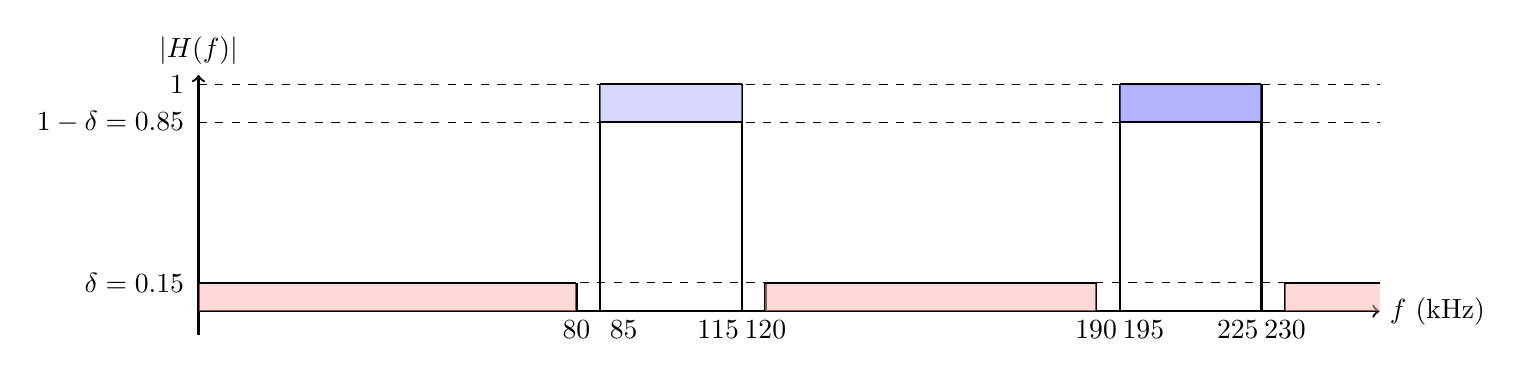
\begin{tikzpicture}[scale=0.06] % Adjust scale as needed
        % Axes
        \draw[thick, ->] (0,0) -- (250,0) node[right] {$f$ (kHz)};
        \draw[thick, ->] (0,-5) -- (0,50) node[above] {$|H(f)|$};
    
        % Frequency points (dashed lines)
        \draw[thick] (80,0) -- (80,6);
        \draw[thick] (85,0) -- (85,48);
        \draw[thick] (115,0) -- (115,48);
        \draw[thick] (120,0) -- (120,6);
        \draw[thick] (190,0) -- (190,6);
        \draw[thick] (195,0) -- (195,48);
        \draw[thick] (225,0) -- (225,48);
        \draw[thick] (230,0) -- (230,6);
    
        \draw[dashed] (0,6) -- (250,6);
        \draw[dashed] (0,40) -- (250,40);
        \draw[dashed] (0,48) -- (250,48);
        
        % Labels for frequency points
        \node[below] at (80,0) {$80$};
        \node[below] at (90,0) {$85$};
        \node[below] at (110,0) {$115$};
        \node[below] at (120,0) {$120$};
        \node[below] at (190,0) {$190$};
        \node[below] at (200,0) {$195$};
        \node[below] at (220,0) {$225$};
        \node[below] at (230,0) {$230$};
    
        % Passband and stopband regions
        \fill[blue!30, opacity=0.5] (85,40) -- (115,40) -- (115,48) -- (85,48) -- cycle;  % Group I passband
        \fill[blue!60, opacity=0.5] (195,40) -- (225,40) -- (225,48) -- (195,48) -- cycle;  % Group II passband
        \fill[red!30, opacity=0.5] (0,0) -- (80,0) -- (80,6) -- (0,6) -- cycle;
        \fill[red!30, opacity=0.5] (120,0) -- (190,0) -- (190,6) -- (120,6) -- cycle;
        \fill[red!30, opacity=0.5] (230,0) -- (250,0) -- (250,6) -- (230,6) -- cycle;
    
        % Filter response
        \draw[thick] (0,6) -- (80,6); % Initial stopband
        \draw[thick] (85,40) -- (115,40); % Group I passband
        \draw[thick] (85,48) -- (115, 48);
        \draw[thick] (120,6) -- (190,6); % Stopband between groups
        \draw[thick] (195,40) -- (225,40); % Group II passband
        \draw[thick] (195,48) -- (225,48);
        \draw[thick] (230,6) -- (250,6); % Final stopband
    
        % Stopband and passband Labels
        \node[left] at (-1,6) {$\delta=0.15$};
        \node[left] at (-1,40) {$1 - \delta=0.85$};
        \node[left] at (-1,48) {$1$};
    \end{tikzpicture}
    \caption{Desired Frequency Response}
    \label{fig:1}
\end{figure}


Now, it should be noted that, the blue regions represents the equiripple / oscillatory passband and the red region represents the monotonic stopband. It should also be noted that, since this is an IIR filter, the upper band is capped to 1.\\
The light blue region, on the left, corresponds to the Group I of frequency bands, while the slightly darker region on the right, corresponds to the Group II of frequency bands.\\



\subsection{Realization of the Frequency Response}
The filter response can be realised by cascading a BandPass Filter with a BandPass Filter \textit{(Series Connection)} OR by adding the result obtained by two BandPass Filters \textit{(Parallel Connection)}. For the purpose of this assignment, we will be using the Cascading option.\\

\begin{figure}[h!]
    \centering
    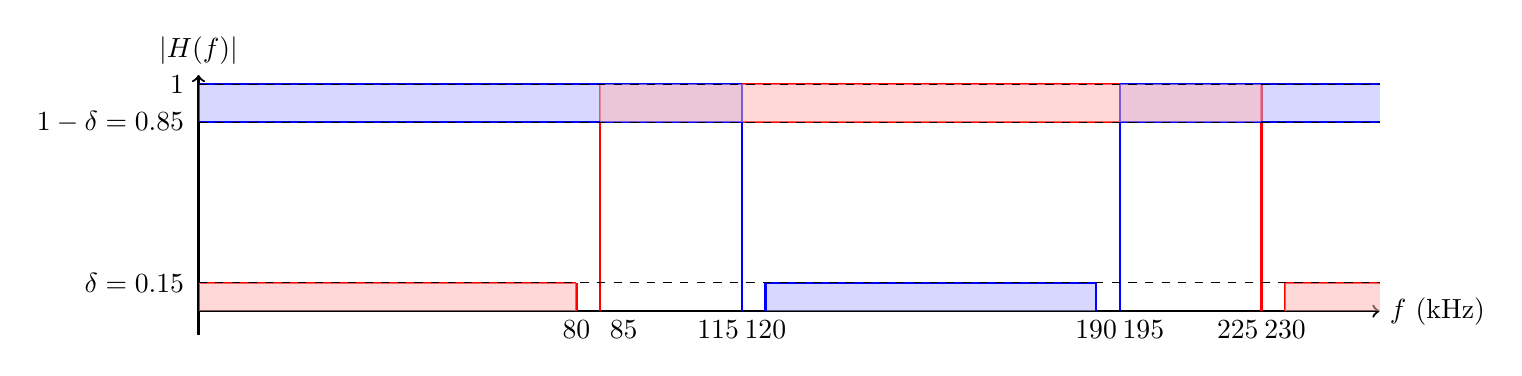
\begin{tikzpicture}[scale=0.06] % Adjust scale as needed
        % Axes
        \draw[thick, ->] (0,0) -- (250,0) node[right] {$f$ (kHz)};
        \draw[thick, ->] (0,-5) -- (0,50) node[above] {$|H(f)|$};
    
        % BandPass Filter
        \draw[thick, red] (80,0) -- (80,6);
        \draw[thick, red] (0,6) -- (80,6);
        \draw[thick, red] (85,0) -- (85,48);
        \draw[thick, red] (85,40) -- (225,40);
        \draw[thick, red] (85,48) -- (225,48);
        \draw[thick, red] (225,0) -- (225,48);
        \draw[thick, red] (230,0) -- (230,6);
        \draw[thick, red] (230,6) -- (250,6);      
        \fill[blue!30, opacity=0.5] (120,0) -- (190,0) -- (190,6) -- (120,6) -- cycle;
        \fill[blue!30, opacity=0.5] (0,40) -- (0,48) -- (115,48) -- (115,40) -- cycle;
        \fill[blue!30, opacity=0.5] (195,40) -- (250,40) -- (250,48) -- (195,48) -- cycle;
        
    
        % BandStop Filter
        \draw[thick, blue] (0,40) -- (115,40);
        \draw[thick, blue] (0,48) -- (115,48);
        \draw[thick, blue] (115,0) -- (115,48);
        \draw[thick, blue] (120,0) -- (120,6);
        \draw[thick, blue] (120,6) -- (190,6);
        \draw[thick, blue] (190,0) -- (190,6);
        \draw[thick, blue] (195,0) -- (195,48);
        \draw[thick, blue] (195,40) -- (250,40);
        \draw[thick, blue] (195,48) -- (250,48); 
        \fill[red!30, opacity=0.5] (85,40) -- (225,40) -- (225,48) -- (85,48) -- cycle;
        \fill[red!30, opacity=0.5] (0,0) -- (80,0) -- (80,6) -- (0,6) -- cycle;
        \fill[red!30, opacity=0.5] (230,0) -- (250,0) -- (250,6) -- (230,6) -- cycle;
    
        
        % Marking the y-axis points
        \draw[dashed] (0,6) -- (250,6);
        \draw[dashed] (0,40) -- (250,40);
        \draw[dashed] (0,48) -- (250,48);
        
        % Labels for frequency points
        \node[below] at (80,0) {$80$};
        \node[below] at (90,0) {$85$};
        \node[below] at (110,0) {$115$};
        \node[below] at (120,0) {$120$};
        \node[below] at (190,0) {$190$};
        \node[below] at (200,0) {$195$};
        \node[below] at (220,0) {$225$};
        \node[below] at (230,0) {$230$};
    
        % Stopband and passband Labels
        \node[left] at (-1,6) {$\delta=0.15$};
        \node[left] at (-1,40) {$1 - \delta=0.85$};
        \node[left] at (-1,48) {$1$};
    \end{tikzpicture}
    \caption{Cascade of BandPass and BandStop Filters}
    \label{fig:2}
\end{figure}

The Blue filter represents the \textcolor{blue}{BandStop Filter} with \textcolor{blue}{stop band from 120kHz to 190kHz}, and 5kHz transition band, across the stopband. The red filter represents the \textcolor{red}{BandPass Filter} with \textcolor{red}{passband between 85kHz and 225kHz}, with a transition band of 5kHz across the passband. \\

\newpage
\section{Designing Filter}
We now require to design the BandPass and BandStop Filter ony by one, to realise the final filter.
\begin{enumerate}
    \item 
        BandPass Filter
        \begin{enumerate}
            \item Passband Range Required: 85kHz - 225kHz
            \item PassBand Tolerance (arbitrary): $\delta_1$
            \item StopBand Tolerance (arbitrary): $\delta_2$
            \item passband Tolerance: 5kHz
        \end{enumerate}
    \item 
        BandStop Filter
        \begin{enumerate}
            \item Passband Range Required: 120kHz - 190kHz
            \item PassBand Tolerance (arbitrary): $\delta_3$
            \item StopBand Tolerance (arbitrary): $\delta_4$
            \item stopband Tolerance: 5kHz
        \end{enumerate}
\end{enumerate}
After cascading the two filters; following will be the value of tolerances and the respective frequency range:
\[
    Tolerances =
    \begin{cases} 
        \delta_2(1-\delta_3), & 0^+ \leq f < 80kHz \\
        (1-\delta_1)(1-\delta_3), & 85kHz \leq f < 115kHz \\
        \delta_4(1-\delta_3), & 120kHz \leq f < 190kHz \\
        (1-\delta_1)(1-\delta_3), & 195kHz \leq f < 225kHz \\
        \delta_2(1-\delta_3), & 230kHz \leq f < 315kHz\\
    \end{cases}
\]
Comparing the Tolerances from the above table to the Tolerance level values from Figure - 1. 
Equating for 85kHz $\leq$ f $\leq$ 115kHz and 195kHz $\leq$ f $\leq$ 225kHz:
\[
    (1-\delta_1)(1-\delta_3) = 1- \delta = 0.85
\]
\[
    1 - \delta_1 - \delta_3 - \delta_1\delta_3 = 0.85
\]
\[
    \delta_1 + \delta_3 - \delta_1 \delta_3 = 0.15
\]
Equating for 0kHz $\leq$ f $\leq$ 80kHz and 230kHz $\leq$ f $\leq$ 315kHz:
\[
    \delta_2 ( 1- \delta_3) = \delta = 0.15 
\]
But equating for 120kHz $\leq$ f $\leq$ 190kHz gives us:
\[
    \delta_4 ( 1- \delta_1) = \delta = 0.15
\]
For the ease of solving, we can assume: $\delta_1$ = $\delta_3$ and $\delta_2$ = $\delta_4$. Thus the above equations become:
\[
    \delta_1 + \delta_3 - \delta_1 \delta_3 = 2\delta_1 - \delta_1^2 = 0.15
\]
Solving the quadratic equation, 
\[
    \delta_1 = \frac{+2 \pm \sqrt{(-2)^2 - 4(1)(0.15)}}{2*1}
\]
Thus, $\delta_1$ can either be 1.92 or 0.08, but we know that $\delta_1$ can't take a value more than 1, thus, $\delta_1$ = 0.08 = $\delta_3$\\
Similarly,
\[
    \delta_2 ( 1- \delta_3) = 0.15
\]
\[
    \delta_2 = \frac{0.15}{0.92} = 0.16 = \delta_4
\]
\subsection{Normalizing the Frequency}
To normalize the frequency, so that the range of frequencies lie between -$\pi$ and +$\pi$. We can use the below formula:
\[
    \omega = \frac{\Omega \cdot 2\pi}{\Omega_{sampling}} = \frac{\Omega\cdot\pi}{315\cdot 10^3}
\]
\subsection{Converting the values to analog}
We can convert these values by using the below formula:
\[
    \Omega = tan(\frac{\omega}{2})
\]

\subsection{Tabulated Values}
Below is the table to convert between the formulas:
\begin{table}[h]
    \centering
    \renewcommand{\arraystretch}{1.3}
    \begin{tabular}{|l|c|c|c|c|c|c|c|c|} \hline
        f(kHz) & 80 & 85 & 115 & 120 & 190 & 195 & 225 & 230 \\ \hline
        Normalized Frequency ($\omega$) & $0.25\pi$ & $0.27\pi$ & $0.365\pi$ & $0.38\pi$ & $0.60\pi$ & $0.62\pi$ & $0.71\pi$ & $0.73\pi$ \\ \hline
        Analog Equivalent ($\Omega$) & 0.41 & 0.45 & 0.645 & 0.68 & 1.38 & 1.47 & 2.04 & 2.21 \\ \hline
    \end{tabular}
    \caption{Frequency values and their corresponding normalized and analog equivalents}
\end{table}

\subsection{Calculating BandPass Filter Analog Characteristics}
Below is the expected Filter value for the BandPass Filter.\\
\begin{figure}[h!]
    \centering
    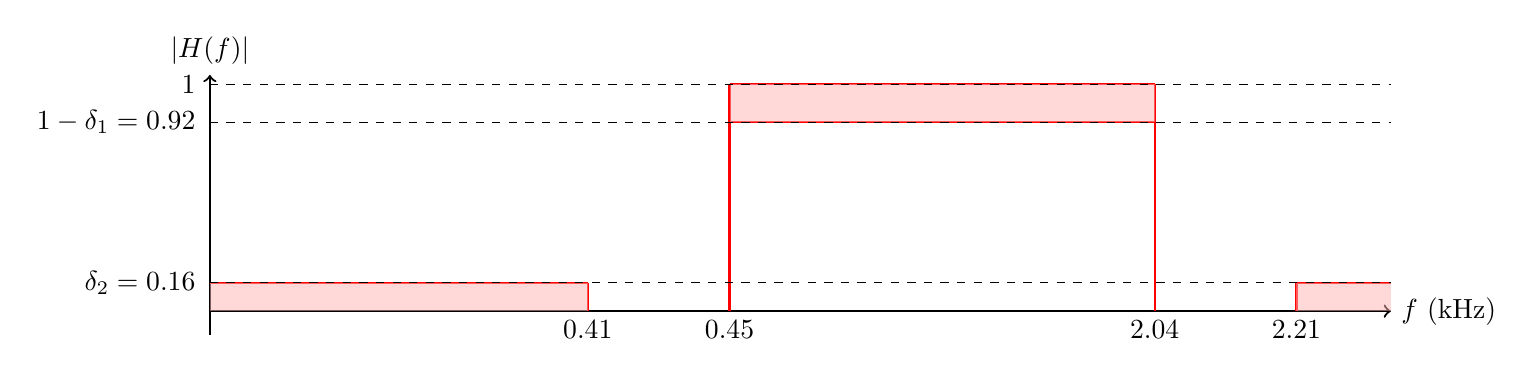
\begin{tikzpicture}[scale=0.06] % Adjust scale as needed
        % Axes
        \draw[thick, ->] (0,0) -- (250,0) node[right] {$f$ (kHz)};
        \draw[thick, ->] (0,-5) -- (0,50) node[above] {$|H(f)|$};
    
        % BandPass Filter
        \draw[thick, red] (80,0) -- (80,6);
        \draw[thick, red] (0,6) -- (80,6);
        \draw[thick, red] (110,0) -- (110,48);
        \draw[thick, red] (110,40) -- (200,40);
        \draw[thick, red] (110,48) -- (200,48);
        \draw[thick, red] (200,0) -- (200,48);
        \draw[thick, red] (230,0) -- (230,6);
        \draw[thick, red] (230,6) -- (250,6);      
        % \fill[blue!30, opacity=0.5] (120,0) -- (190,0) -- (190,6) -- (120,6) -- cycle;
        % \fill[blue!30, opacity=0.5] (0,40) -- (0,48) -- (115,48) -- (115,40) -- cycle;
        % \fill[blue!30, opacity=0.5] (195,40) -- (250,40) -- (250,48) -- (195,48) -- cycle;
        
    
        % BandStop Filter
        % \draw[thick, blue] (0,40) -- (115,40);
        % \draw[thick, blue] (0,48) -- (115,48);
        % \draw[thick, blue] (115,0) -- (115,48);
        % \draw[thick, blue] (120,0) -- (120,6);
        % \draw[thick, blue] (120,6) -- (190,6);
        % \draw[thick, blue] (190,0) -- (190,6);
        % \draw[thick, blue] (195,0) -- (195,48);
        % \draw[thick, blue] (195,40) -- (250,40);
        % \draw[thick, blue] (195,48) -- (250,48); 
        \fill[red!30, opacity=0.5] (110,40) -- (200,40) -- (200,48) -- (110,48) -- cycle;
        \fill[red!30, opacity=0.5] (0,0) -- (80,0) -- (80,6) -- (0,6) -- cycle;
        \fill[red!30, opacity=0.5] (230,0) -- (250,0) -- (250,6) -- (230,6) -- cycle;
    
        
        % Marking the y-axis points
        \draw[dashed] (0,6) -- (250,6);
        \draw[dashed] (0,40) -- (250,40);
        \draw[dashed] (0,48) -- (250,48);
        
        % Labels for frequency points
        \node[below] at (80,0) {$0.41$};
        % \node[below] at (90,0) {$0.45$};
        \node[below] at (110,0) {$0.45$};
        % \node[below] at (120,0) {$120$};
        % \node[below] at (190,0) {$190$};
        \node[below] at (200,0) {$2.04$};
        % \node[below] at (220,0) {$2.04$};
        \node[below] at (230,0) {$2.21$};
    
        % Stopband and passband Labels
        \node[left] at (-1,6) {$\delta_2=0.16$};
        \node[left] at (-1,40) {$1 - \delta_1=0.92$};
        \node[left] at (-1,48) {$1$};
    \end{tikzpicture}
    \caption{Desired BandPass Filters (Not drawn to Scale)}
    \label{fig:3}
\end{figure}
\\Using the result for converting a Bandpass filter to Chebyshev LPF; as taught in class on "10th February 2025 (Monday) (L-16)". \\
\[
    \Omega_L = \frac{\Omega^2 - \Omega_0^2}{B\Omega}
\]
\[
    \Omega_0^2 = \Omega_{p1} \Omega_{p2}
\]
\[
    B = \Omega_{p2} - \Omega_{p1}
\]
\newpage
The below is the filter response of a typical bandpass filter:
\begin{figure}[h!]
    \centering
    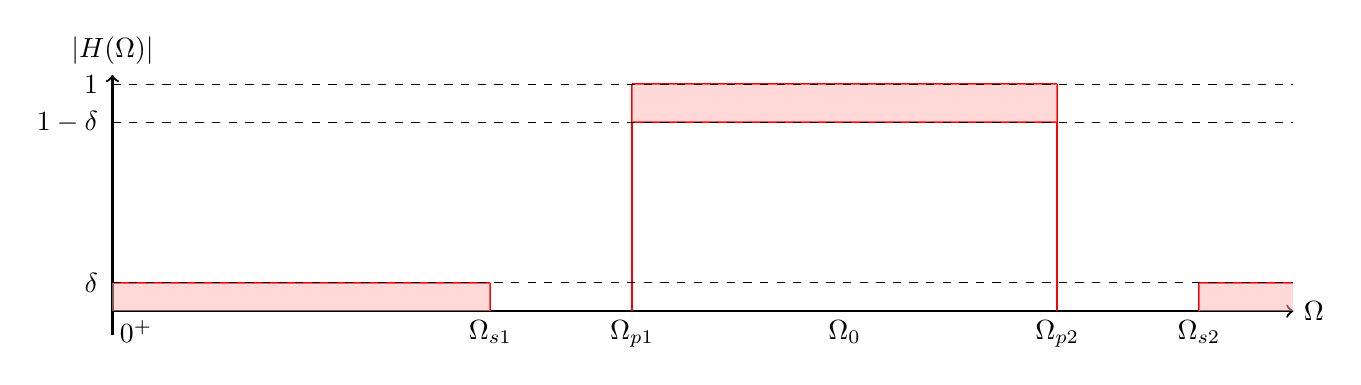
\begin{tikzpicture}[scale=0.06] % Adjust scale as needed
        % Axes
        \draw[thick, ->] (0,0) -- (250,0) node[right] {$\Omega$};
        \draw[thick, ->] (0,-5) -- (0,50) node[above] {$|H(\Omega)|$};
    
        % BandPass Filter
        \draw[thick, red] (80,0) -- (80,6);
        \draw[thick, red] (0,6) -- (80,6);
        \draw[thick, red] (110,0) -- (110,48);
        \draw[thick, red] (110,40) -- (200,40);
        \draw[thick, red] (110,48) -- (200,48);
        \draw[thick, red] (200,0) -- (200,48);
        \draw[thick, red] (230,0) -- (230,6);
        \draw[thick, red] (230,6) -- (250,6);
        \fill[red!30, opacity=0.5] (110,40) -- (200,40) -- (200,48) -- (110,48) -- cycle;
        \fill[red!30, opacity=0.5] (0,0) -- (80,0) -- (80,6) -- (0,6) -- cycle;
        \fill[red!30, opacity=0.5] (230,0) -- (250,0) -- (250,6) -- (230,6) -- cycle;
    
        
        % Marking the y-axis points
        \draw[dashed] (0,6) -- (250,6);
        \draw[dashed] (0,40) -- (250,40);
        \draw[dashed] (0,48) -- (250,48);
        
        % Labels for frequency points
        \node[below] at (5, 0) {$0^+$};
        \node[below] at (80,0) {$\Omega_{s1}$};
        \node[below] at (110,0) {$\Omega_{p1}$};
        \node[below] at (155,0) {$\Omega_0$};
        \node[below] at (200,0) {$\Omega_{p2}$};
        \node[below] at (230,0) {$\Omega_{s2}$};
    
        % Stopband and passband Labels
        \node[left] at (-1,6) {$\delta$};
        \node[left] at (-1,40) {$1 - \delta$};
        \node[left] at (-1,48) {$1$};
    \end{tikzpicture}
    \caption{Frequency Response of a typical BandPass Filters}
    \label{fig:4}
\end{figure}
\\After the above operation on the filter response, the below LPF is obtained:
\begin{figure}[h!]
    \centering
    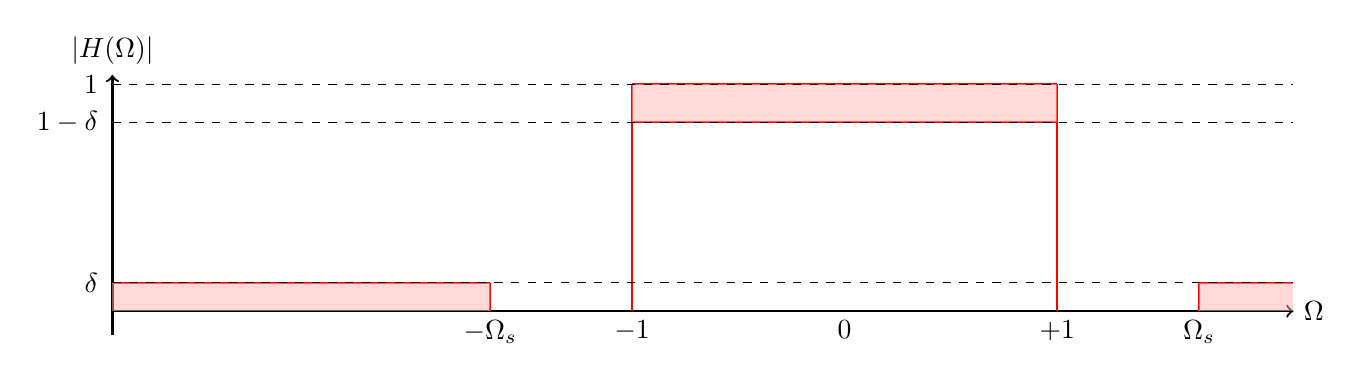
\begin{tikzpicture}[scale=0.06] % Adjust scale as needed
        % Axes
        \draw[thick, ->] (0,0) -- (250,0) node[right] {$\Omega$};
        \draw[thick, ->] (0,-5) -- (0,50) node[above] {$|H(\Omega)|$};
    
        % BandPass Filter
        \draw[thick, red] (80,0) -- (80,6);
        \draw[thick, red] (0,6) -- (80,6);
        \draw[thick, red] (110,0) -- (110,48);
        \draw[thick, red] (110,40) -- (200,40);
        \draw[thick, red] (110,48) -- (200,48);
        \draw[thick, red] (200,0) -- (200,48);
        \draw[thick, red] (230,0) -- (230,6);
        \draw[thick, red] (230,6) -- (250,6);
        \fill[red!30, opacity=0.5] (110,40) -- (200,40) -- (200,48) -- (110,48) -- cycle;
        \fill[red!30, opacity=0.5] (0,0) -- (80,0) -- (80,6) -- (0,6) -- cycle;
        \fill[red!30, opacity=0.5] (230,0) -- (250,0) -- (250,6) -- (230,6) -- cycle;
    
        
        % Marking the y-axis points
        \draw[dashed] (0,6) -- (250,6);
        \draw[dashed] (0,40) -- (250,40);
        \draw[dashed] (0,48) -- (250,48);
        
        % Labels for frequency points
        % \node[below] at (5, 0) {$0^+$};
        \node[below] at (80,0) {$ - \Omega_{s}$};
        \node[below] at (110,0) {$-1$};
        \node[below] at (155,0) {$0$};
        \node[below] at (200,0) {$+1$};
        \node[below] at (230,0) {$\Omega_{s}$};
    
        % Stopband and passband Labels
        \node[left] at (-1,6) {$\delta$};
        \node[left] at (-1,40) {$1 - \delta$};
        \node[left] at (-1,48) {$1$};
    \end{tikzpicture}
    \caption{Frequency Response of a typical BandPass Filters}
    \label{fig:4}
\end{figure}
\\Comparing the graphs of Figure 5 and Figure 4 and equating the respective values, we obtain:
\[
    \Omega_{s1} = 0.41; \Omega_{s2} = 2.21
\]
\[
    \Omega_{p1} = 0.45; \Omega_{p2} = 2.04
\]
Substituting the above values of $\Omega_{p1}$ and $\Omega_{p2}$ into the formulae of $\Omega_L$: 
\[
    \Omega_L = \frac{\Omega^2 - (0.45)(2.04)}{\Omega\cdot(2.04 - 0.45)} = \frac{\Omega^2 - 0.918}{1.59\Omega}
\]
Also, $\Omega_{p2}$ gets mapped to +1, $\Omega_{p1}$ gets mapped to -1. $\Omega_{s1}$ gets mapped to $\Omega_{Ls1}$ while $\Omega_{s2}$ gets mapped to $\Omega_{Ls2}$. We can calculate the values of $\Omega_{Ls1}$ and $\Omega_{Ls2}$:
\[
    \Omega_{Ls1}(\Omega) = \Omega_{Ls1}(0.41) = \frac{(0.41)^2 - 0.918}{0.41\cdot 1.59} = -1.15
\]
\[
    \Omega_{Ls2}(\Omega) = \Omega_{Ls2}(2.21) = \frac{(2.21)^2 - 0.918}{2.21\cdot 1.59} = 1.128 \approx 1.13
\]
\subsubsection{Specifications of a Low Pass Filter}
$\Omega_p$ (passband edge) = +1\\
$\Omega_s$ (stopband edge) = min($\Omega_{Ls1}$, $\Omega_{Ls2}$) = min(1.13, 1.15) = 1.13\\
$D_1$ = $\frac{1}{(1-\delta_1)^2} - 1$ = $\frac{1}{0.92^2} - 1$ = 0.18\\
$D_2$ = $\frac{1}{\delta_2^2} - 1$ = $\frac{1}{0.16^2} - 1$ = 38\\
Using the above obtained results to calculate the order of a Chebyshev filter; using information from the \href{https://youtu.be/lM7oEy2s8Fw}{NPTEL 22B Lecture on Youtube as well as NPTEL website}\\
\[
    N = \ceil[\Bigg]{\frac{cosh^{-1}(+\sqrt{\frac{D_2}{D_1}})}{cosh^{-1}(\frac{\Omega_s}{\Omega_p})}}
\]
\[
    N \geq \ceil[\Bigg]{\frac{cosh^{-1}(+\sqrt{\frac{38}{0.18}})}{cosh^{-1}(\frac{1.13}{1})}} = \ceil[\Bigg]{\frac{3.368}{0.504}} = \ceil[\Bigg]{6.675} = 7
\]
Since, we choose the minimum possible value of N to save resources, the \textbf{Order of the Chebyshev Filter is 7}.
% \subsubsection{Write in the Laplace form}
% \[
%     H_{analog, LPF1}(s) = 1/\left(1 + \left(\frac{s_L}{\Omega_c}\right)^2\right)
% \]
% \[
%     \frac{\Omega_p}{(D_1)^{\frac{1}{2N}}} \leq \Omega_c \leq 
% \]

\subsection{Calculating BandStop Filter Analog Characteristics}
Below is the expected Filter Response required for the Design.\\
\begin{figure}[h!]
    \centering
    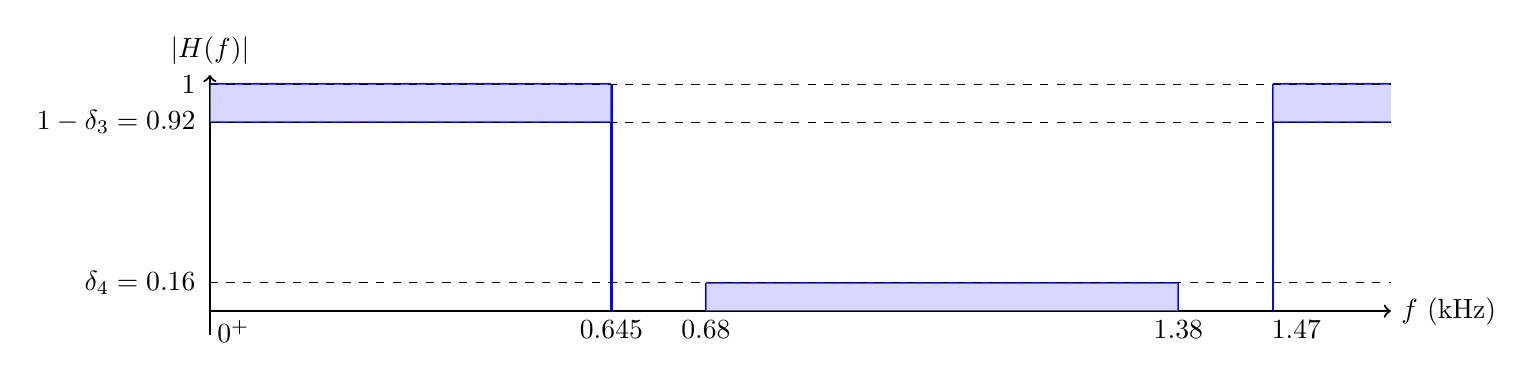
\begin{tikzpicture}[scale=0.06] % Adjust scale as needed
        % Axes
        \draw[thick, ->] (0,0) -- (250,0) node[right] {$f$ (kHz)};
        \draw[thick, ->] (0,-5) -- (0,50) node[above] {$|H(f)|$};

        % BandStop Filter
        \draw[thick, blue] (0,40) -- (85,40);
        \draw[thick, blue] (0,48) -- (85,48);
        \draw[thick, blue] (85,0) -- (85,48);
        \draw[thick, blue] (105,0) -- (105,6);
        \draw[thick, blue] (105,6) -- (205,6);
        \draw[thick, blue] (205,0) -- (205,6);
        \draw[thick, blue] (225,0) -- (225,48);
        \draw[thick, blue] (225,40) -- (250,40);
        \draw[thick, blue] (225,48) -- (250,48); 
        \fill[blue!30, opacity=0.5] (105,0) -- (205,0) -- (205,6) -- (105,6) -- cycle;
        \fill[blue!30, opacity=0.5] (0,40) -- (0,48) -- (85,48) -- (85,40) -- cycle;
        \fill[blue!30, opacity=0.5] (225,40) -- (250,40) -- (250,48) -- (225,48) -- cycle;
    
        
        % Marking the y-axis points
        \draw[dashed] (0,6) -- (250,6);
        \draw[dashed] (0,40) -- (250,40);
        \draw[dashed] (0,48) -- (250,48);
        
        % Labels for frequency points
        \node[below] at (5,0) {$0^+$};
        \node[below] at (85,0) {$0.645$};
        \node[below] at (105,0) {$0.68$};
        \node[below] at (205,0) {$1.38$};
        \node[below] at (230,0) {$1.47$};
    
        % Stopband and passband Labels
        \node[left] at (-1,6) {$\delta_4=0.16$};
        \node[left] at (-1,40) {$1 - \delta_3=0.92$};
        \node[left] at (-1,48) {$1$};
    \end{tikzpicture}
    \caption{Desired BandStop Filters (Not drawn to Scale)}
    \label{fig:6}
\end{figure}
\\Using the result for converting a Bandstop filter to Chebyshev LPF; as taught in class on "10th February 2025 (Monday) (L-16)". \\
\[
    \Omega_L = \frac{B\Omega}{\Omega_0^2 - \Omega^2}
\]
\[
    B = \Omega_{p2} - \Omega_{p1}
\]
\[
    \Omega_0^2 = \Omega_{p1}\Omega_{p2}
\]
The below is the filter response of a typical bandpass filter:
\begin{figure}[h!]
    \centering
    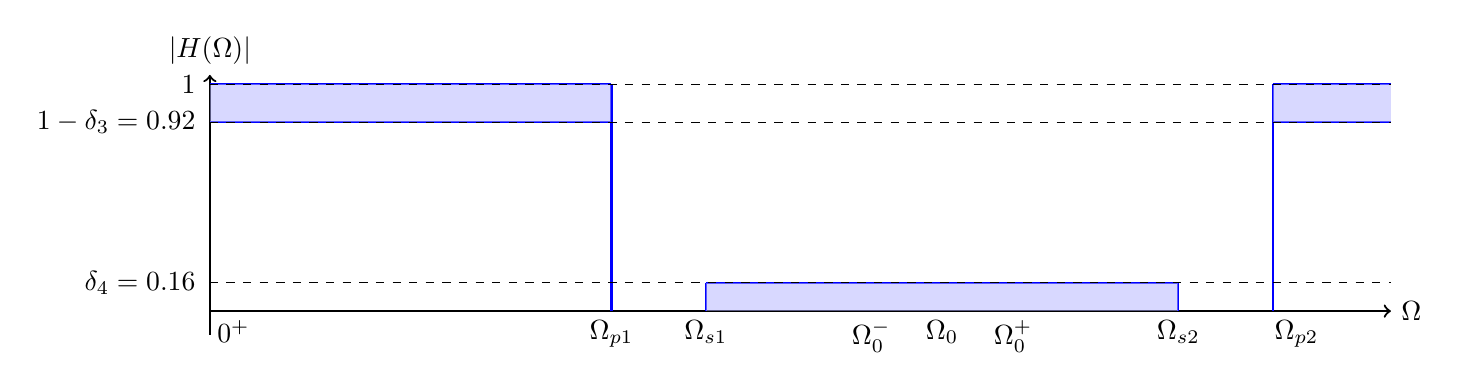
\begin{tikzpicture}[scale=0.06] % Adjust scale as needed
        % Axes
        \draw[thick, ->] (0,0) -- (250,0) node[right] {$\Omega$};
        \draw[thick, ->] (0,-5) -- (0,50) node[above] {$|H(\Omega)|$};

        % BandStop Filter
        \draw[thick, blue] (0,40) -- (85,40);
        \draw[thick, blue] (0,48) -- (85,48);
        \draw[thick, blue] (85,0) -- (85,48);
        \draw[thick, blue] (105,0) -- (105,6);
        \draw[thick, blue] (105,6) -- (205,6);
        \draw[thick, blue] (205,0) -- (205,6);
        \draw[thick, blue] (225,0) -- (225,48);
        \draw[thick, blue] (225,40) -- (250,40);
        \draw[thick, blue] (225,48) -- (250,48); 
        \fill[blue!30, opacity=0.5] (105,0) -- (205,0) -- (205,6) -- (105,6) -- cycle;
        \fill[blue!30, opacity=0.5] (0,40) -- (0,48) -- (85,48) -- (85,40) -- cycle;
        \fill[blue!30, opacity=0.5] (225,40) -- (250,40) -- (250,48) -- (225,48) -- cycle;
    
        
        % Marking the y-axis points
        \draw[dashed] (0,6) -- (250,6);
        \draw[dashed] (0,40) -- (250,40);
        \draw[dashed] (0,48) -- (250,48);
        
        % Labels for frequency points
        \node[below] at (5,0) {$0^+$};
        \node[below] at (85,0) {$\Omega_{p1}$};
        \node[below] at (105,0) {$\Omega_{s1}$};
        \node[below] at (140,0) {$\Omega_0^-$};
        \node[below] at (155,0) {$\Omega_0$};
        \node[below] at (170,0) {$\Omega_0^+$};
        \node[below] at (205,0) {$\Omega_{s2}$};
        \node[below] at (230,0) {$\Omega_{p2}$};
    
        % Stopband and passband Labels
        \node[left] at (-1,6) {$\delta_4=0.16$};
        \node[left] at (-1,40) {$1 - \delta_3=0.92$};
        \node[left] at (-1,48) {$1$};
    \end{tikzpicture}
    \caption{Frequency of a typical Bandstop filter}
    \label{fig:6}
\end{figure}
\\After the above operation on the filter response, the below LPF is obtained:
\newpage
\begin{figure}[h!]
    \centering
    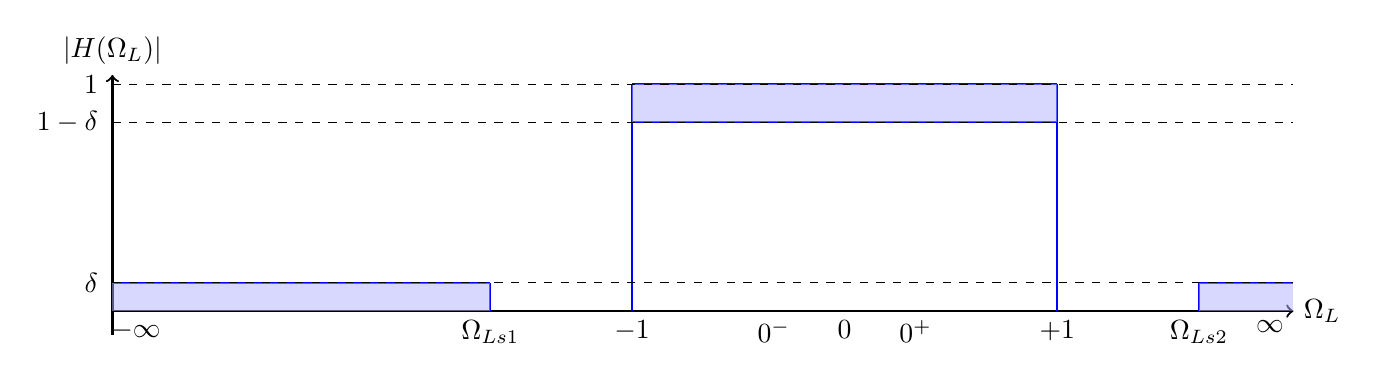
\begin{tikzpicture}[scale=0.06] % Adjust scale as needed
        % Axes
        \draw[thick, ->] (0,0) -- (250,0) node[right] {$\Omega_L$};
        \draw[thick, ->] (0,-5) -- (0,50) node[above] {$|H(\Omega_L)|$};
    
        % BandPass Filter
        \draw[thick, blue] (80,0) -- (80,6);
        \draw[thick, blue] (0,6) -- (80,6);
        \draw[thick, blue] (110,0) -- (110,48);
        \draw[thick, blue] (110,40) -- (200,40);
        \draw[thick, blue] (110,48) -- (200,48);
        \draw[thick, blue] (200,0) -- (200,48);
        \draw[thick, blue] (230,0) -- (230,6);
        \draw[thick, blue] (230,6) -- (250,6);
        \fill[blue!30, opacity=0.5] (110,40) -- (200,40) -- (200,48) -- (110,48) -- cycle;
        \fill[blue!30, opacity=0.5] (0,0) -- (80,0) -- (80,6) -- (0,6) -- cycle;
        \fill[blue!30, opacity=0.5] (230,0) -- (250,0) -- (250,6) -- (230,6) -- cycle;
    
        
        % Marking the y-axis points
        \draw[dashed] (0,6) -- (250,6);
        \draw[dashed] (0,40) -- (250,40);
        \draw[dashed] (0,48) -- (250,48);
        
        % Labels for frequency points
        \node[below] at (5, 0) {$-\infty$};
        \node[below] at (80,0) {$\Omega_{Ls1}$};
        \node[below] at (110,0) {$-1$};
        \node[below] at (140,0) {$0^-$};
        \node[below] at (155,0) {$0$};
        \node[below] at (170,0) {$0^+$};
        \node[below] at (200,0) {$+1$};
        \node[below] at (230,0) {$\Omega_{Ls2}$};
        \node[below] at (245,0) {$\infty$};
    
        % Stopband and passband Labels
        \node[left] at (-1,6) {$\delta$};
        \node[left] at (-1,40) {$1 - \delta$};
        \node[left] at (-1,48) {$1$};
    \end{tikzpicture}
    \caption{Frequency Response of a typical Lowpass Filters}
    \label{fig:8}
\end{figure}
Unlike the BandPass filter, this one typically doesn't follow a one-to-one mapping, instead it follows the below mapping:
\begin{table}[h]
    \centering
    \renewcommand{\arraystretch}{1.3}
    \begin{tabular}{|l|c|c|c|c|c|c|c|c|c|}
        \hline
        \textbf{$\Omega$} & $\Omega_0^+$ & $\Omega_{s2}$ & $\Omega_{p2}$ & $+\infty$ & $\Omega_0$ & $0^+$ & $\Omega_{p1}$ & $\Omega_{s1}$ & $\Omega_0^-$ \\ \hline
        \textbf{$\Omega_L$} & $-\infty$ & $\Omega_{Ls2}$ & -1 & $0^-$ & 0 & $0^+$ & 1 & $\Omega_{Ls1}$ & +$\infty$ \\ \hline
    \end{tabular}
    \caption{Conversion from BandStop to LPF}
    \label{tab:freq_values}
\end{table}
Comparing the values from Figure 7 and Figure 8:
\[
    \Omega_{s1} = 0.68; \Omega_{s2} = 1.38
\]
\[
    \Omega_{p1} = 0.645; \Omega_{p2} = 1.47
\]
\[
    \Omega_0^2 = \Omega_{p1} \cdot \Omega_{p2} = 0.645 \cdot 1.47 = 0.94815
\]
\[
    B = \Omega_{p2} - \Omega_{p1} = 1.47 - 0.645 = 0.825
\]
\[
    \Omega_{Ls1}(\Omega) = \Omega_{Ls1}(0.68) = \frac{0.825\cdot 0.68}{0.94815 - (0.68)^2} = 1.154 \approx 1.15
\]
\[
    \Omega_{Ls2}(\Omega) = \Omega_{Ls2}(1.38) = \frac{0.825\cdot 1.38}{0.94815 - (1.38)^2} = -1.19
\]


\subsubsection{Specifications of a Low Pass Filter}
$\Omega_p$ (passband edge) = +1\\
$\Omega_s$ (stopband edge) = min($\Omega_{Ls1}$, $\Omega_{Ls2}$) = min(1.15, 1.19) = 1.15\\
$D_1$ = $\frac{1}{(1-\delta_1)^2} - 1$ = $\frac{1}{0.92^2} - 1$ = 0.18\\
$D_2$ = $\frac{1}{\delta_2^2} - 1$ = $\frac{1}{0.16^2} - 1$ = 38\\
Using the above obtained results to calculate the order of a Chebyshev filter; using information from the \href{https://youtu.be/lM7oEy2s8Fw}{NPTEL 22B Lecture on Youtube as well as NPTEL website}\\
\[
    N = \ceil[\Bigg]{\frac{cosh^{-1}(+\sqrt{\frac{D_2}{D_1}})}{cosh^{-1}(\frac{\Omega_s}{\Omega_p})}}
\]
\[
    N \geq \ceil[\Bigg]{\frac{cosh^{-1}(+\sqrt{\frac{38}{0.18}})}{cosh^{-1}(\frac{1.15}{1})}} = \ceil[\Bigg]{\frac{3.368}{0.541}} = \ceil[\Bigg]{6.224} = 7
\]
Since, we choose the minimum possible value of N to save resources, the \textbf{Order of the Chebyshev Filter is 7}.


\section{Manual Calculation for Poles}
We know that the roots of a chebysehv filter are given by:
\[
    s_k = \sigma_k + j\Omega_k
\]
\[
    \sigma_k = - a\cdot sin\frac{(2k + 1) \pi}{2N}
\]
\[
    \Omega_k = b\cdot cos\frac{(2k + 1) \pi}{2N}
\]
\[
    s_k = - sinh(\frac{1}{N}\cdot sinh^{-1}\frac{1}{\epsilon}) \cdot sin\frac{(2k + 1) \pi}{2N} + j \cdot cosh(\frac{1}{N}\cdot sinh^{-1}\frac{1}{\epsilon}) \cdot cos\frac{(2k + 1) \pi}{2N}
\]

\subsection{BandPass Filter}
\begin{table}[h]
    \centering
    \renewcommand{\arraystretch}{1.3}
    \begin{tabular}{|l|c|} \hline
        $\Omega_s$ & 1.13 \\ \hline
        $\Omega_p$ & 1 \\ \hline
        $\epsilon (= \sqrt{D_1})$ & $0.18^{0.5} = 0.424$ \\ \hline
        $D_2$ & 38 \\ \hline
        N (Number of Poles) & 7 \\ \hline
        a ( = $sinh(\frac{1}{N}\cdot sinh^{-1}\frac{1}{\epsilon})$ & 0.229\\ \hline
        b ( = $cosh(\frac{1}{N}\cdot sinh^{-1}\frac{1}{\epsilon})$ & 1.026 \\ \hline
    \end{tabular}
    % \caption{Frequency values and their corresponding normalized and analog equivalents}
\end{table}
\subsection{BandStop Filter}
\begin{table}[h]
    \centering
    \renewcommand{\arraystretch}{1.3}
    \begin{tabular}{|l|c|} \hline
        $\Omega_s$ & 1.15 \\ \hline
        $\Omega_p$ & 1 \\ \hline
        $\epsilon (= \sqrt{D_1})$ & $0.18^{0.5} = 0.424$ \\ \hline
        $D_2$ & 38 \\ \hline
        N (Number of Poles) & 7 \\ \hline
        a ( = $sinh(\frac{1}{N}\cdot sinh^{-1}\frac{1}{\epsilon})$ & 0.229\\ \hline
        b ( = $cosh(\frac{1}{N}\cdot sinh^{-1}\frac{1}{\epsilon})$ & 1.026 \\ \hline
    \end{tabular}
    % \caption{Frequency values and their corresponding normalized and analog equivalents}
\end{table}
\subsection{Poles Calculation}
Since the value of N and $\Omega_p = 1$ is same, the poles will remain same. Thus, poles are given by:\\
For N = 7, k will vary from k = 0 to k = 6. \\
\[
    s_k = -0.229\cdot sin\left(\frac{(2k+1)\pi}{14}\right) + j\cdot 1.026\cdot cos\left(\frac{(2k+1)\pi}{14}\right)
\]
\[
s_0 = -0.229\cdot \sin\left(\frac{\pi}{14}\right) + j\cdot 1.026\cdot \cos\left(\frac{\pi}{14}\right)
\]

\[
s_1 = -0.229\cdot \sin\left(\frac{3\pi}{14}\right) + j\cdot 1.026\cdot \cos\left(\frac{3\pi}{14}\right)
\]

\[
s_2 = -0.229\cdot \sin\left(\frac{5\pi}{14}\right) + j\cdot 1.026\cdot \cos\left(\frac{5\pi}{14}\right)
\]

\[
s_3 = -0.229\cdot \sin\left(\frac{7\pi}{14}\right) + j\cdot 1.026\cdot \cos\left(\frac{7\pi}{14}\right)
\]

\[
s_4 = -0.229\cdot \sin\left(\frac{9\pi}{14}\right) + j\cdot 1.026\cdot \cos\left(\frac{9\pi}{14}\right)
\]

\[
s_5 = -0.229\cdot \sin\left(\frac{11\pi}{14}\right) + j\cdot 1.026\cdot \cos\left(\frac{11\pi}{14}\right)
\]

\[
s_6 = -0.229\cdot \sin\left(\frac{13\pi}{14}\right) + j\cdot 1.026\cdot \cos\left(\frac{13\pi}{14}\right)
\]
\\
The system function is given by:
\[
    H(s) = \frac{K}{\Pi_{k} (s-s_k)} = \frac{K}{D_N(s)}
\]
To find \( K \) for odd value of N, we use the given formula:

\[
K = D_N(s) \Big|_{s=0}
\]

where \( D_N(s) \) is the denominator of the system function:

\[
D_N(s) = \prod_{k=0}^{N-1} (s - s_k)
\]

For \( N = 7 \), we substitute \( s = 0 \):

\[
K = \prod_{k=0}^{6} (0 - s_k) = (-1)^7 \prod_{k=0}^{6} s_k
\]

Since \( (-1)^7 = -1 \), we get:

\[
K = - \prod_{k=0}^{6} s_k
\]

Each \( s_k \) is given by:

\[
s_k = -0.229\cdot \sin\left(\frac{(2k+1)\pi}{14}\right) + j\cdot 1.026\cdot \cos\left(\frac{(2k+1)\pi}{14}\right)
\]

Thus, the computed value of \( K \) is:

\[
K \approx 0.0367
\]
\[
    H(s) = \frac{0.0367}{\Pi_k(s-s_k)}
\]

\newpage
\begin{figure}[h!]
    \centering
    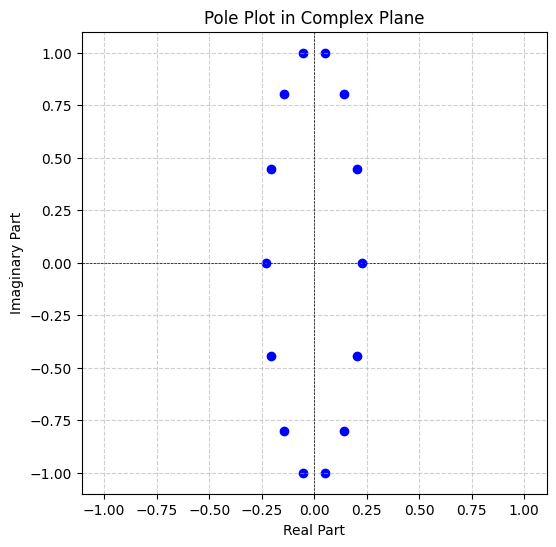
\includegraphics[width=0.6\linewidth]{./Optional_Images/Poles_Plot.png}
    \caption{Plot of Chebyshev Filter for BandPass / BandStop Filter (They have the same poles in this case)}
    \label{fig:enter-label}
\end{figure}

\subsection{Filter Response for BandPass Filter}
\[
    f(x) = \frac{1 - e^{-ix}}{1 + e^{-ix}}
\]
\[
\frac{\prod_{k=0}^{6} \left( -i \cos\left(\frac{(2k+1) \pi}{14}\right) \cosh(0.227540122101) + \sin\left(\frac{(2k+1) \pi}{14}\right) \sinh(0.227540122101) \right)}
{\prod_{k=0}^{6} \left( \frac{\left(f(x)\right)^2 + 0.918}{1.59 \cdot f(x)} - i \cos\left(\frac{(2k+1) \pi}{14}\right) \cosh(0.227540122101) + \sin\left(\frac{(2k+1) \pi}{14}\right) \sinh(0.227540122101) \right)}
\]
\begin{figure}[h!]
    \centering
    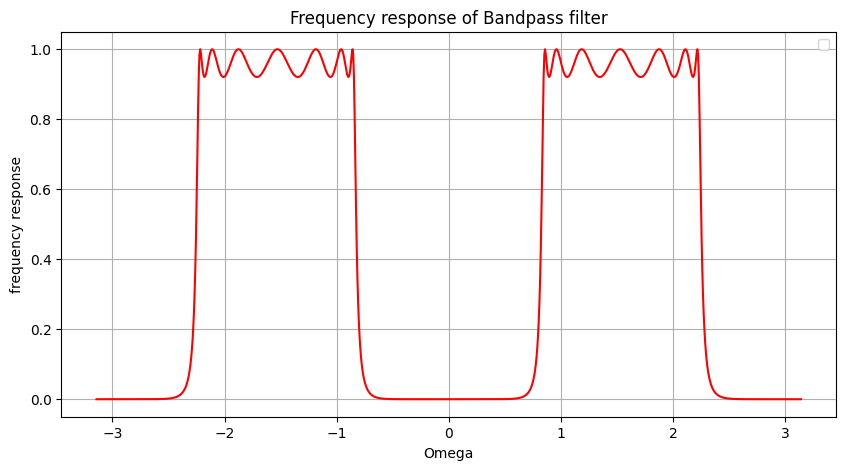
\includegraphics[width=1\linewidth]{./Optional_Images/BandPass_Filter_Response.png}
    \caption{Plot of Filter Response for BandPass Filter}
    \label{fig:enter-label}
\end{figure}

\newpage
\subsection{Filter Response for BandStop Filter}
\[
    f(x) = \frac{1 - e^{-ix}}{1 + e^{-ix}}
\]
\[
\frac{\prod_{k=0}^{6} \left( -i \cos\left(\frac{(2k+1) \pi}{14}\right) \cosh(0.227540122101) + \sin\left(\frac{(2k+1) \pi}{14}\right) \sinh(0.227540122101) \right)}
{\prod_{k=0}^{6} \left( \frac{0.825 \cdot f(x)}{\left(f(x)\right)^2 + 0.94815} - i \cos\left(\frac{(2k+1) \pi}{14}\right) \cosh(0.227540122101) + \sin\left(\frac{(2k+1) \pi}{14}\right) \sinh(0.227540122101) \right)}
\]
\begin{figure}[h!]
    \centering
    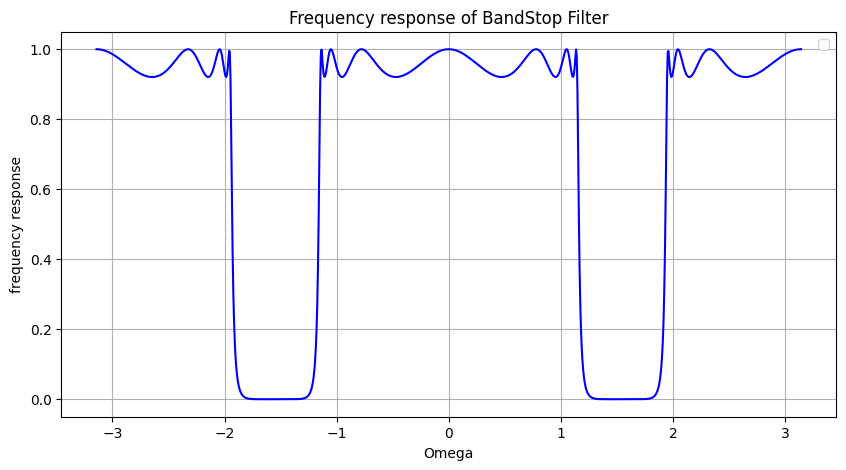
\includegraphics[width=1\linewidth]{./Optional_Images/BandStop_Filter_Response.png}
    \caption{Plot of Filter Response for BandStop Filter}
    \label{fig:enter-label}
\end{figure}

\subsection{Filter Response for Cascaded Filter}
\begin{figure}[h!]
    \centering
    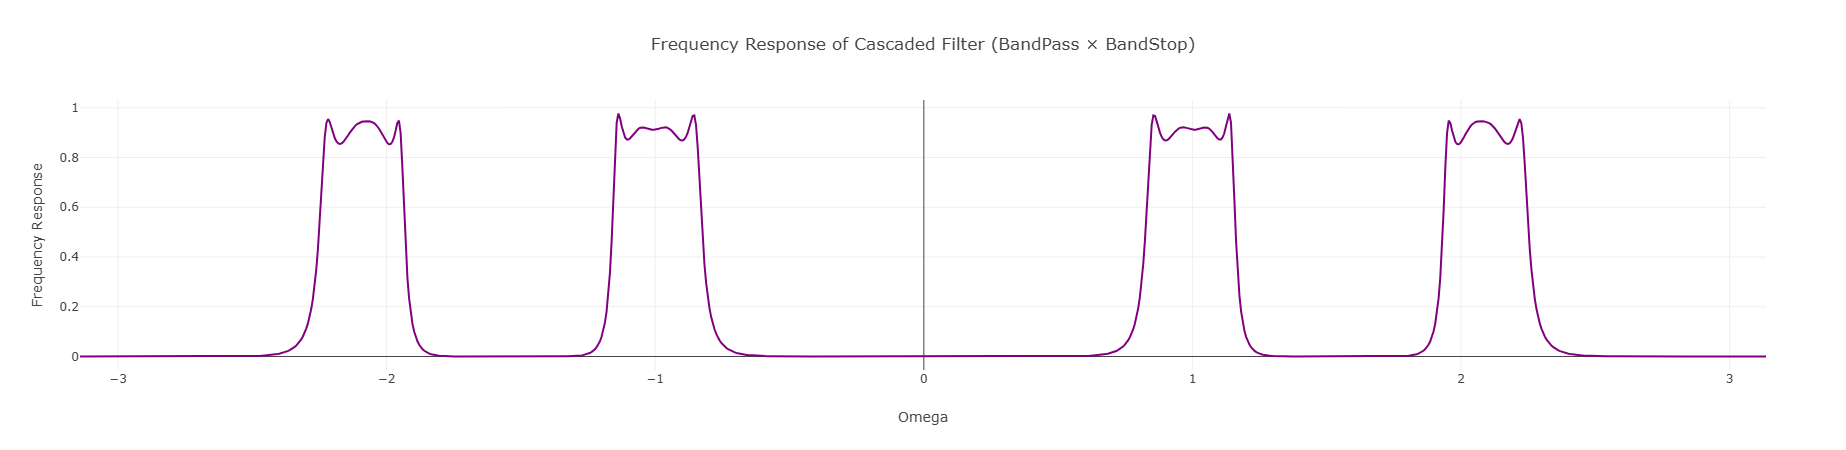
\includegraphics[width=1\linewidth]{./Optional_Images/Cascaded_Filter_Response.png}
    \caption{Plot of Filter Response for Cascaded Filter}
    \label{fig:enter-label}
\end{figure}


\newpage 
\section{Code for Poles Plot and Filter Response Plot}
The following section provides the code used to generate the plots in Python.

\subsection{JavaScript Code for Poles Plot}
\begin{lstlisting}[language=HTML, caption=Filter Type Definition]
function plotPoles() {
    const A_values = [-0.229, 0.229];
    const B = 1.026;
    let theta = Array.from({length: 7}, (_, k) => (Math.PI * (2 * k + 1)) / 14);
    let poles = [];

    A_values.forEach(A => {
        theta.forEach(t => {
            let realPart = A * Math.sin(t);
            let imagPart = B * Math.cos(t);
            poles.push({x: realPart, y: imagPart});
        });
    });

    let trace = {
        x: poles.map(p => p.x),
        y: poles.map(p => p.y),
        mode: 'markers',
        marker: { color: 'blue', size: 8 },
        type: 'scatter'
    };

    let layout = {
        title: 'Pole Plot in Complex Plane',
        xaxis: { title: 'Real Part', zeroline: true, scaleanchor: "y" },
        yaxis: { title: 'Imaginary Part', zeroline: true },
        showlegend: false
    };

    Plotly.newPlot('pole-plot', [trace], layout);
}

plotPoles();
\end{lstlisting}

\subsection{JavaScript Code for BandPass Filter Response}
\begin{lstlisting}[language=HTML, caption=Filter Type Definition]
window.onload = function () {
    console.log("Math.js Loaded:", typeof math !== "undefined");
    console.log("Plotly Loaded:", typeof Plotly !== "undefined");

    if (typeof math === "undefined" || typeof Plotly === "undefined") {
        alert("Error: Math.js or Plotly.js failed to load. Check your internet connection.");
        return;
    }

    function BandPassFilter(x) {
        let Numerator = math.complex(1, 0);
        let Denominator = math.complex(1, 0);

        for (let k = 0; k < 7; k++) {
            let angle = (2 * k + 1) * Math.PI / 14;
            let term1 = math.multiply(
                math.complex(0, -1), 
                math.multiply(Math.cos(angle), 
                Math.cosh(0.227540122101)));
            let term2 = math.multiply(Math.sin(angle), Math.sinh(0.227540122101));

            let exponent = math.exp(math.multiply(math.complex(0, -1), x));
            let fraction = math.divide(math.subtract(1, exponent), math.add(1, exponent));

            let term3 = math.divide(math.add(math.pow(fraction, 2), 0.918), math.multiply(1.59, fraction));

            Numerator = math.multiply(Numerator, math.add(term1, term2));
            Denominator = math.multiply(Denominator, math.subtract(math.subtract(term3, term1), term2));
        }

        return math.divide(Numerator, Denominator);
    }

    // Values on the x-axis
    let x_values = math.range(-Math.PI, Math.PI, 2 * Math.PI / 1000).toArray();
    
    // BandPass Filter Response
    let y_bandpass = x_values.map(x => BandPassFilter(x));
    let mag_bandpass = y_bandpass.map(y => math.abs(y));

    let trace1 = {
        x: x_values,
        y: mag_bandpass,
        mode: 'lines',
        line: { color: 'red' },
        name: 'BandPass Magnitude'
    };

    let layout1 = {
        title: "Frequency Response of BandPass Filter",
        xaxis: { title: "Omega" },
        yaxis: { title: "Frequency Response" },
        grid: { visible: true }
    };

    Plotly.newPlot("bandpass-plot", [trace1], layout1);
};
\end{lstlisting}

\subsection{JavaScript Code for BandStop Filter}
\begin{lstlisting}[language=HTML, caption=Filter Type Definition]
window.onload = function () {
    console.log("Math.js Loaded:", typeof math !== "undefined");
    console.log("Plotly Loaded:", typeof Plotly !== "undefined");

    if (typeof math === "undefined" || typeof Plotly === "undefined") {
        alert("Error: Math.js or Plotly.js failed to load. Check your internet connection.");
        return;
    }

    function BandStopFilter(x) {
        let Numerator = math.complex(1, 0);
        let Denominator = math.complex(1, 0);

        for (let k = 0; k < 7; k++) {
            let angle = (2 * k + 1) * Math.PI / 14;
            let term1 = math.multiply(math.complex(0, -1), math.multiply(Math.cos(angle), Math.cosh(0.227540122101)));
            let term2 = math.multiply(Math.sin(angle), Math.sinh(0.227540122101));

            let exponent = math.exp(math.multiply(math.complex(0, -1), x));
            let fraction = math.divide(math.subtract(1, exponent), math.add(1, exponent));

            let term3 = math.divide(math.multiply(0.825, fraction), math.add(math.pow(fraction, 2), 0.94815));

            Numerator = math.multiply(Numerator, math.add(term1, term2));
            Denominator = math.multiply(Denominator, math.subtract(math.add(term3, term2), term1));
        }

        return math.divide(Numerator, Denominator);
    }

    // Values on the x-axis
    let x_values = math.range(-Math.PI, Math.PI, 2 * Math.PI / 1000).toArray();
        
    // BandStop Filter Response
    let y_bandstop = x_values.map(x => BandStopFilter(x));
    let mag_bandstop = y_bandstop.map(y => math.abs(y));
    
    let trace2 = {
        x: x_values,
        y: mag_bandstop,
        mode: 'lines',
        line: { color: 'blue' },
        name: 'BandStop Magnitude'
    };

    let layout2 = {
        title: "Frequency Response of BandStop Filter",
        xaxis: { title: "Omega" },
        yaxis: { title: "Frequency Response" },
        grid: { visible: true }
    };

    Plotly.newPlot("bandstop-plot", [trace2], layout2);
};
\end{lstlisting}


\subsection{JavaScript Code for Cascaded Filter Response}
\begin{lstlisting}[language=HTML, caption=Filter Type Definition]
window.onload = function () {
    console.log("Math.js Loaded:", typeof math !== "undefined");
    console.log("Plotly Loaded:", typeof Plotly !== "undefined");

    if (typeof math === "undefined" || typeof Plotly === "undefined") {
        alert("Error: Math.js or Plotly.js failed to load. Check your internet connection.");
        return;
    }
    
    // Values on the x-axis
    let x_values = math.range(-Math.PI, Math.PI, 2 * Math.PI / 1000).toArray();
    // Cascaded Filter Response
    let y_cascaded = y_bandpass.map((bp, i) => math.multiply(bp, y_bandstop[i]));
    let mag_cascaded = y_cascaded.map(y => math.abs(y));

    let trace3 = {
        x: x_values,
        y: mag_cascaded,
        mode: 'lines',
        line: { color: 'purple' },
        name: 'Cascaded Filter Magnitude'
    };

    let layout3 = {
        title: "Frequency Response of Cascaded Filter (BandPass × BandStop)",
        xaxis: { title: "Omega" },
        yaxis: { title: "Frequency Response" },
        grid: { visible: true }
    };

    Plotly.newPlot("cascaded-plot", [trace3], layout3);
};
\end{lstlisting}

\subsection{Combined JavaScript Code for Filter Response}
\begin{lstlisting}[language=HTML, caption=Filter Type Definition]
<!DOCTYPE html>
<html lang="en">
<head>
    <meta charset="UTF-8">
    <meta name="viewport" content="width=device-width, initial-scale=1.0">
    <title>Filter Frequency Response</title>
    <script src="https://cdnjs.cloudflare.com/ajax/libs/mathjs/11.3.2/math.js" defer></script>
    <script src="https://cdn.plot.ly/plotly-2.20.0.min.js" defer></script>
</head>
<body>

<h2>Frequency Response of BandPass Filter</h2>
<div id="bandpass-plot"></div>

<h2>Frequency Response of BandStop Filter</h2>
<div id="bandstop-plot"></div>

<h2>Frequency Response of Cascaded Filter (BandPass × BandStop)</h2>
<div id="cascaded-plot"></div>

<script>
    window.onload = function () {
        console.log("Math.js Loaded:", typeof math !== "undefined");
        console.log("Plotly Loaded:", typeof Plotly !== "undefined");

        if (typeof math === "undefined" || typeof Plotly === "undefined") {
            alert("Error: Math.js or Plotly.js failed to load. Check your internet connection.");
            return;
        }

        function BandPassFilter(x) {
            let Numerator = math.complex(1, 0);
            let Denominator = math.complex(1, 0);

            for (let k = 0; k < 7; k++) {
                let angle = (2 * k + 1) * Math.PI / 14;
                let term1 = math.multiply(math.complex(0, -1), math.multiply(Math.cos(angle), Math.cosh(0.227540122101)));
                let term2 = math.multiply(Math.sin(angle), Math.sinh(0.227540122101));

                let exponent = math.exp(math.multiply(math.complex(0, -1), x));
                let fraction = math.divide(math.subtract(1, exponent), math.add(1, exponent));

                let term3 = math.divide(math.add(math.pow(fraction, 2), 0.918), math.multiply(1.59, fraction));

                Numerator = math.multiply(Numerator, math.add(term1, term2));
                Denominator = math.multiply(Denominator, math.subtract(math.subtract(term3, term1), term2));
            }

            return math.divide(Numerator, Denominator);
        }

        function BandStopFilter(x) {
            let Numerator = math.complex(1, 0);
            let Denominator = math.complex(1, 0);

            for (let k = 0; k < 7; k++) {
                let angle = (2 * k + 1) * Math.PI / 14;
                let term1 = math.multiply(math.complex(0, -1), math.multiply(Math.cos(angle), Math.cosh(0.227540122101)));
                let term2 = math.multiply(Math.sin(angle), Math.sinh(0.227540122101));

                let exponent = math.exp(math.multiply(math.complex(0, -1), x));
                let fraction = math.divide(math.subtract(1, exponent), math.add(1, exponent));

                let term3 = math.divide(math.multiply(0.825, fraction), math.add(math.pow(fraction, 2), 0.94815));

                Numerator = math.multiply(Numerator, math.add(term1, term2));
                Denominator = math.multiply(Denominator, math.subtract(math.add(term3, term2), term1));
            }

            return math.divide(Numerator, Denominator);
        }

	// Values on the x-axis
        let x_values = math.range(-Math.PI, Math.PI, 2 * Math.PI / 1000).toArray();
        
	// BandPass Filter Response
	let y_bandpass = x_values.map(x => BandPassFilter(x));
        let mag_bandpass = y_bandpass.map(y => math.abs(y));

	// BandStop Filter Response
        let y_bandstop = x_values.map(x => BandStopFilter(x));
        let mag_bandstop = y_bandstop.map(y => math.abs(y));

	// Cascaded Filter Response
        let y_cascaded = y_bandpass.map((bp, i) => math.multiply(bp, y_bandstop[i]));
        let mag_cascaded = y_cascaded.map(y => math.abs(y));



        let trace1 = {
            x: x_values,
            y: mag_bandpass,
            mode: 'lines',
            line: { color: 'red' },
            name: 'BandPass Magnitude'
        };

        let layout1 = {
            title: "Frequency Response of BandPass Filter",
            xaxis: { title: "Omega" },
            yaxis: { title: "Frequency Response" },
            grid: { visible: true }
        };

        Plotly.newPlot("bandpass-plot", [trace1], layout1);



	let trace2 = {
            x: x_values,
            y: mag_bandstop,
            mode: 'lines',
            line: { color: 'blue' },
            name: 'BandStop Magnitude'
        };

        let layout2 = {
            title: "Frequency Response of BandStop Filter",
            xaxis: { title: "Omega" },
            yaxis: { title: "Frequency Response" },
            grid: { visible: true }
        };

        Plotly.newPlot("bandstop-plot", [trace2], layout2);



        let trace3 = {
            x: x_values,
            y: mag_cascaded,
            mode: 'lines',
            line: { color: 'purple' },
            name: 'Cascaded Filter Magnitude'
        };

        let layout3 = {
            title: "Frequency Response of Cascaded Filter (BandPass × BandStop)",
            xaxis: { title: "Omega" },
            yaxis: { title: "Frequency Response" },
            grid: { visible: true }
        };

        Plotly.newPlot("cascaded-plot", [trace3], layout3);
    };
</script>

</body>
</html>
\end{lstlisting}


\section{Comparison}
This document compares the design characteristics of two types of IIR filters: \textbf{Butterworth} and \textbf{Chebyshev}. The comparison considers parameters such as filter order, passband behavior, stopband characteristics, and computational complexity.

\\
Two filter types are considered:
\begin{itemize}
    \item \textbf{Filter Type 1}: Butterworth Bandpass (Order 22) and Bandstop (Order 19).
    \item \textbf{Filter Type 2}: Chebyshev Bandpass (Order 7) and Bandstop (Order 7).
\end{itemize}

\begin{table}[h]
    \centering
    \renewcommand{\arraystretch}{1.3}
    \begin{tabular}{|l|c|c|}
        \hline
        \textbf{Aspect} & \textbf{Butterworth Filter} & \textbf{Chebyshev Filter} \\
        \hline \hline
        \textbf{Design Approach} & Bandpass (N = 22), Bandstop (N = 19) & Bandpass (N = 7), Bandstop (N = 7) \\
        \hline
        \textbf{Filter Order} & Higher (22/19) – More complexity & Lower (7/7) – Less complexity \\
        \hline
        \textbf{Passband Characteristics} & Maximally flat, no ripples & Equiripple passband (Type I Chebyshev) \\
        \hline
        \textbf{Stopband Characteristics} & Smooth attenuation (monotonic) & Sharper roll-off with ripples \\
        \hline
        \textbf{Transition Band} & Gradual roll-off, requiring high order & Steeper roll-off, lower order suffices \\
        \hline
        \textbf{Computational Complexity} & Higher due to more coefficients & Lower due to fewer coefficients \\
        \hline
        \textbf{Group Delay} & Higher due to high order & Lower but with variations from ripple \\
        \hline
        \textbf{Implementation Feasibility} & More challenging & Easier due to lower order \\
        \hline
    \end{tabular}
    \caption{Comparison of Butterworth and Chebyshev Filters}
    \label{tab:comparison}
\end{table}

\section{Conclusion}
Both filters have their own advantages. The \textbf{Butterworth filter} provides a maximally flat passband with a smooth roll-off but requires a higher order for sharp transitions. The \textbf{Chebyshev filter}, on the other hand, achieves steeper roll-off with a lower order but introduces ripples in the passband and stopband. The choice depends on the application requirements, balancing flatness, roll-off, and computational efficiency.







\section{Peer Review}
\textbf{Name of student:} Anupam Rawat\\
\textbf{Name and Roll Number of the reviewer} : Jatin Kumar 22B3922\\
\textbf{Group Number} : 34\\
\textbf{Review Comments} :\\
I have reviewed the filter design assignment of Anupam Rawat, Roll Number 22B3982. The filter number assigned to him is 104. Following are my comments on his
assignment:\\
He has correctly implemented the filter, and the response are in accordance to the expected frequency response. He has also correctly used the chebyshev approximations to
implement the IIR designs for each filter. He has included all the code, results and their plots in the report.\\

\section*{Acknowledgements}

I would like to express my sincere gratitude to \textbf{Professor V. M. Gadre} for introducing and teaching me the fundamental and profoundly important course on \textit{Digital Signal Processing}. The structured tasks and exercises in this course have greatly enhanced my understanding of various concepts in this field.
\\
Furthermore, I am deeply thankful to my group members, \textbf{Mr. Jatin Kumar} and \textbf{Mr. Rishabh Bhardwaj}, for their unwavering support, insightful discussions, and seamless collaboration throughout this course. Their contributions have been invaluable in refining my learning experience.

\noindent I truly appreciate the guidance and teamwork that is making this journey both enriching and intellectually stimulating.

\end{document}
